\chapter{O Método Simplex}

\section{Origem do Método Simplex}
O método simplex surgiu nos Estados Unidos e foi proposto pelo matemático George Dantzig. Quando trabalhava no Pentágono recebeu dos seus colegas o desafio de tentar mecanizar o processo de planejamento. No ano de 1947 Dantzig propôs o método simplex que tornou possível a solução de problemas de otimização de vários tipos, como transporte, produção, alocação de recursos e problemas de escalonamento \cite{OrigemSimplex}.

\section{Descrição do Método}
\subsection{Princípio Básico do Método}
A idéia do método simplex consiste em resolver repetidas vezes um sistema de equações lineares, e assim obter uma sucessão de soluções até encontrar a solução ótima. Ou seja, é um processo onde nos movemos de uma solução viável para outra sempre melhor ou pelo menos não pior.

Um problema de programação linear é sempre constituído de uma função objetivo e várias restrições. Geometricamente, essas restrições resultam em uma forma geométrica, chamada hiperplano, no espaço n-dimensional sendo n o número de variáveis no modelo. E cada vértice desse hiperplano é considerado uma solução viável, como ilustra o exemplo abaixo.
\begin{center}
	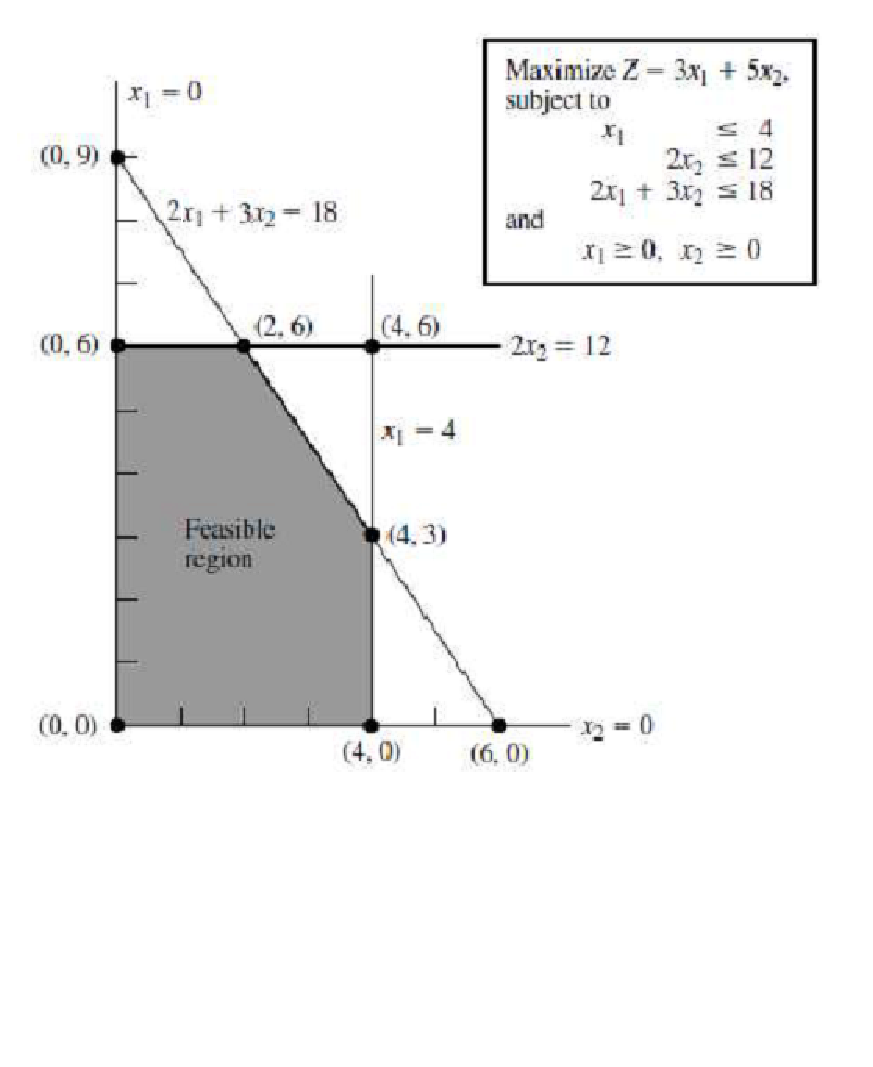
\includegraphics[scale=0.5]{graficos/Simplex_grafico_completo}
	\captionof{figure}{Um modelo de programação linear e a sua respectiva representação gráfica}
\end{center}
